\section{Problem}
 \begin{wrapfigure}{R}{0.22\columnwidth}
\vspace{-5.5em}
		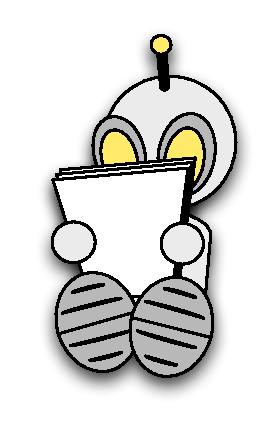
\includegraphics[width=0.2\columnwidth]{diagrams/robot_reading.pdf}
 \end{wrapfigure}

Pathfinding is a problem. Blah blah blah.
Lorem ipsum dolor sit amet, consectetur adipisicing elit, sed do eiusmod
tempor incididunt ut labore et dolore magna aliqua. Ut enim ad minim
veniam, quis nostrud exercitation ullamco laboris nisi ut aliquip ex ea
commodo consequat. Duis aute irure dolor in reprehenderit in voluptate
velit esse cillum dolore eu fugiat nulla pariatur. Excepteur sint occaecat
cupidatat non proident, sunt in culpa qui officia deserunt mollit anim
id est laborum.


Somewhere in the body there's often some maths, which might be an inline equation
line $a^2+b^2=c^2$ and then there are sometimes displayed equations too, like:
 \begin{figure}[h]
	\centering
	\subfigure[On a tile grid each location has up to 4 neighbours.] {
	\label{fig:4cgrid}
		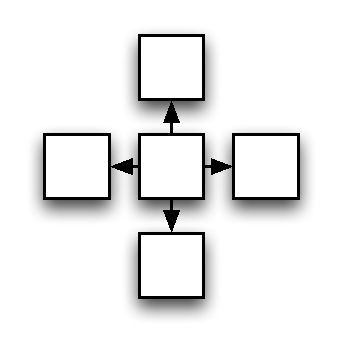
\includegraphics[width=0.45\columnwidth]{diagrams/4c_grid.pdf}
	}
	\subfigure[On an octile grid each location has up to 8 neighbours.] {
	\label{fig:8cgrid}
		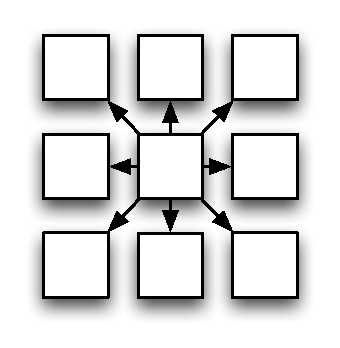
\includegraphics[width=0.45\columnwidth]{diagrams/8c_grid.pdf}
	}
	
	\subfigure[Grid maps are often used for pathfinding in video games.] {
	\label{fig:wc3}
		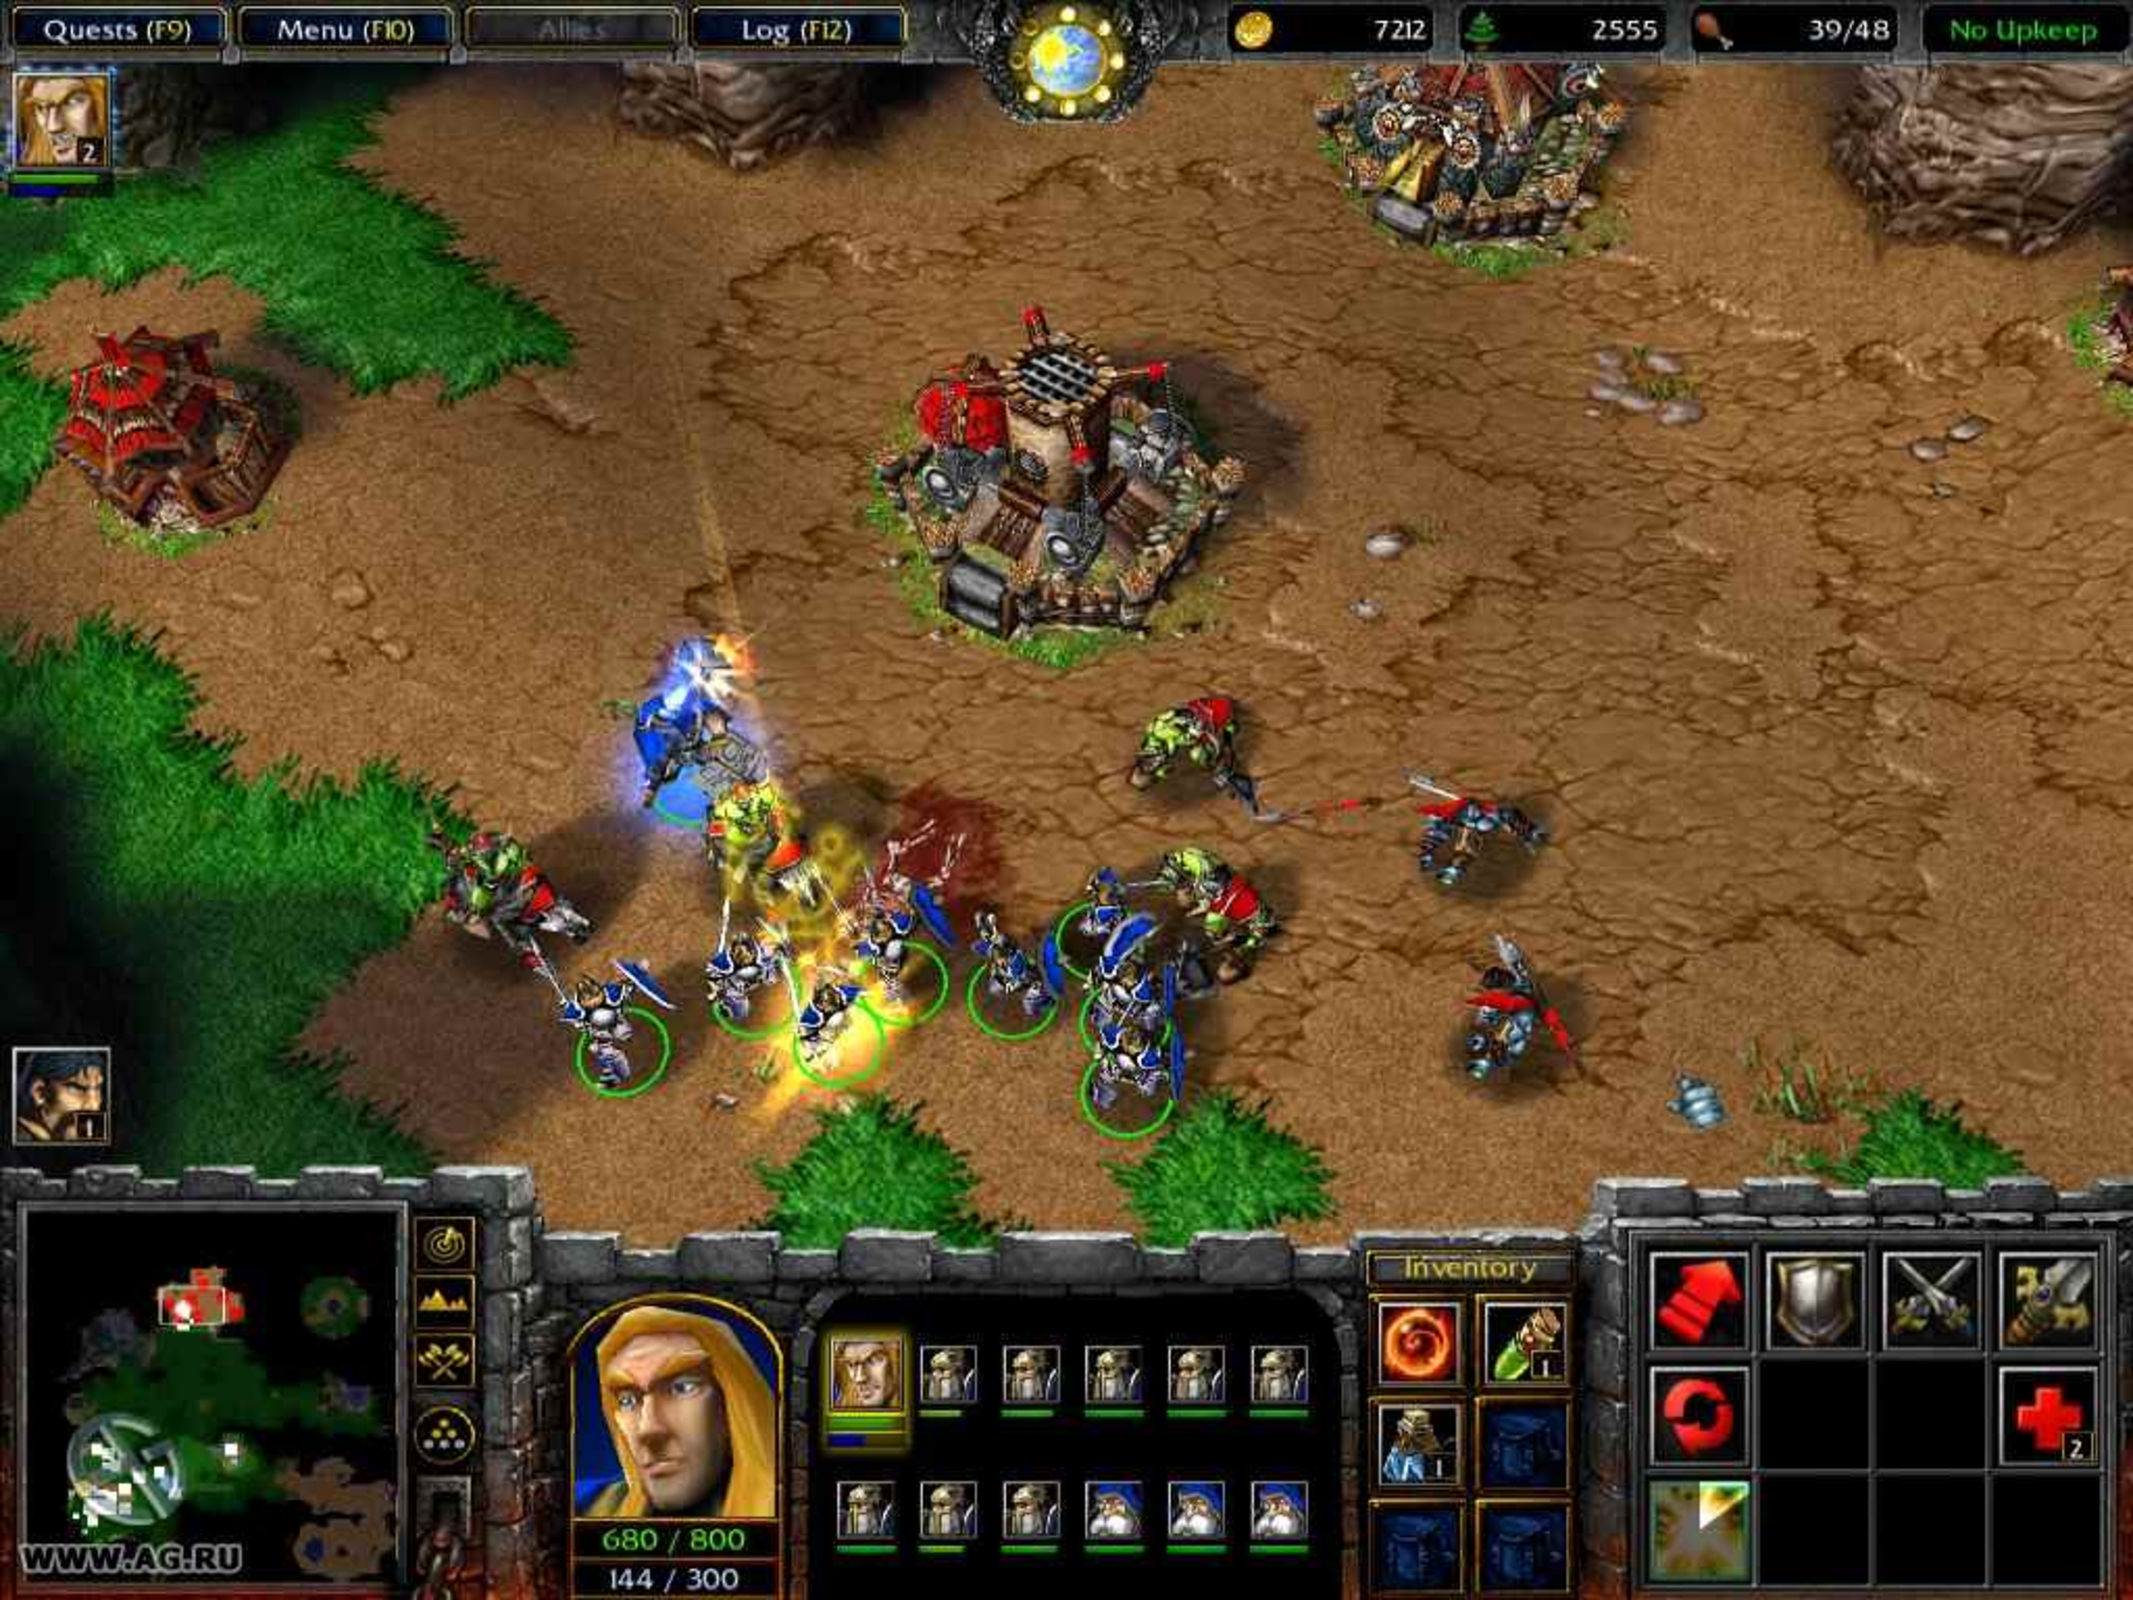
\includegraphics[width=0.45\columnwidth]{diagrams/wc3.pdf}
	}
	\subfigure[Grid maps are also common in robotics.] {
	\label{fig:maze}
		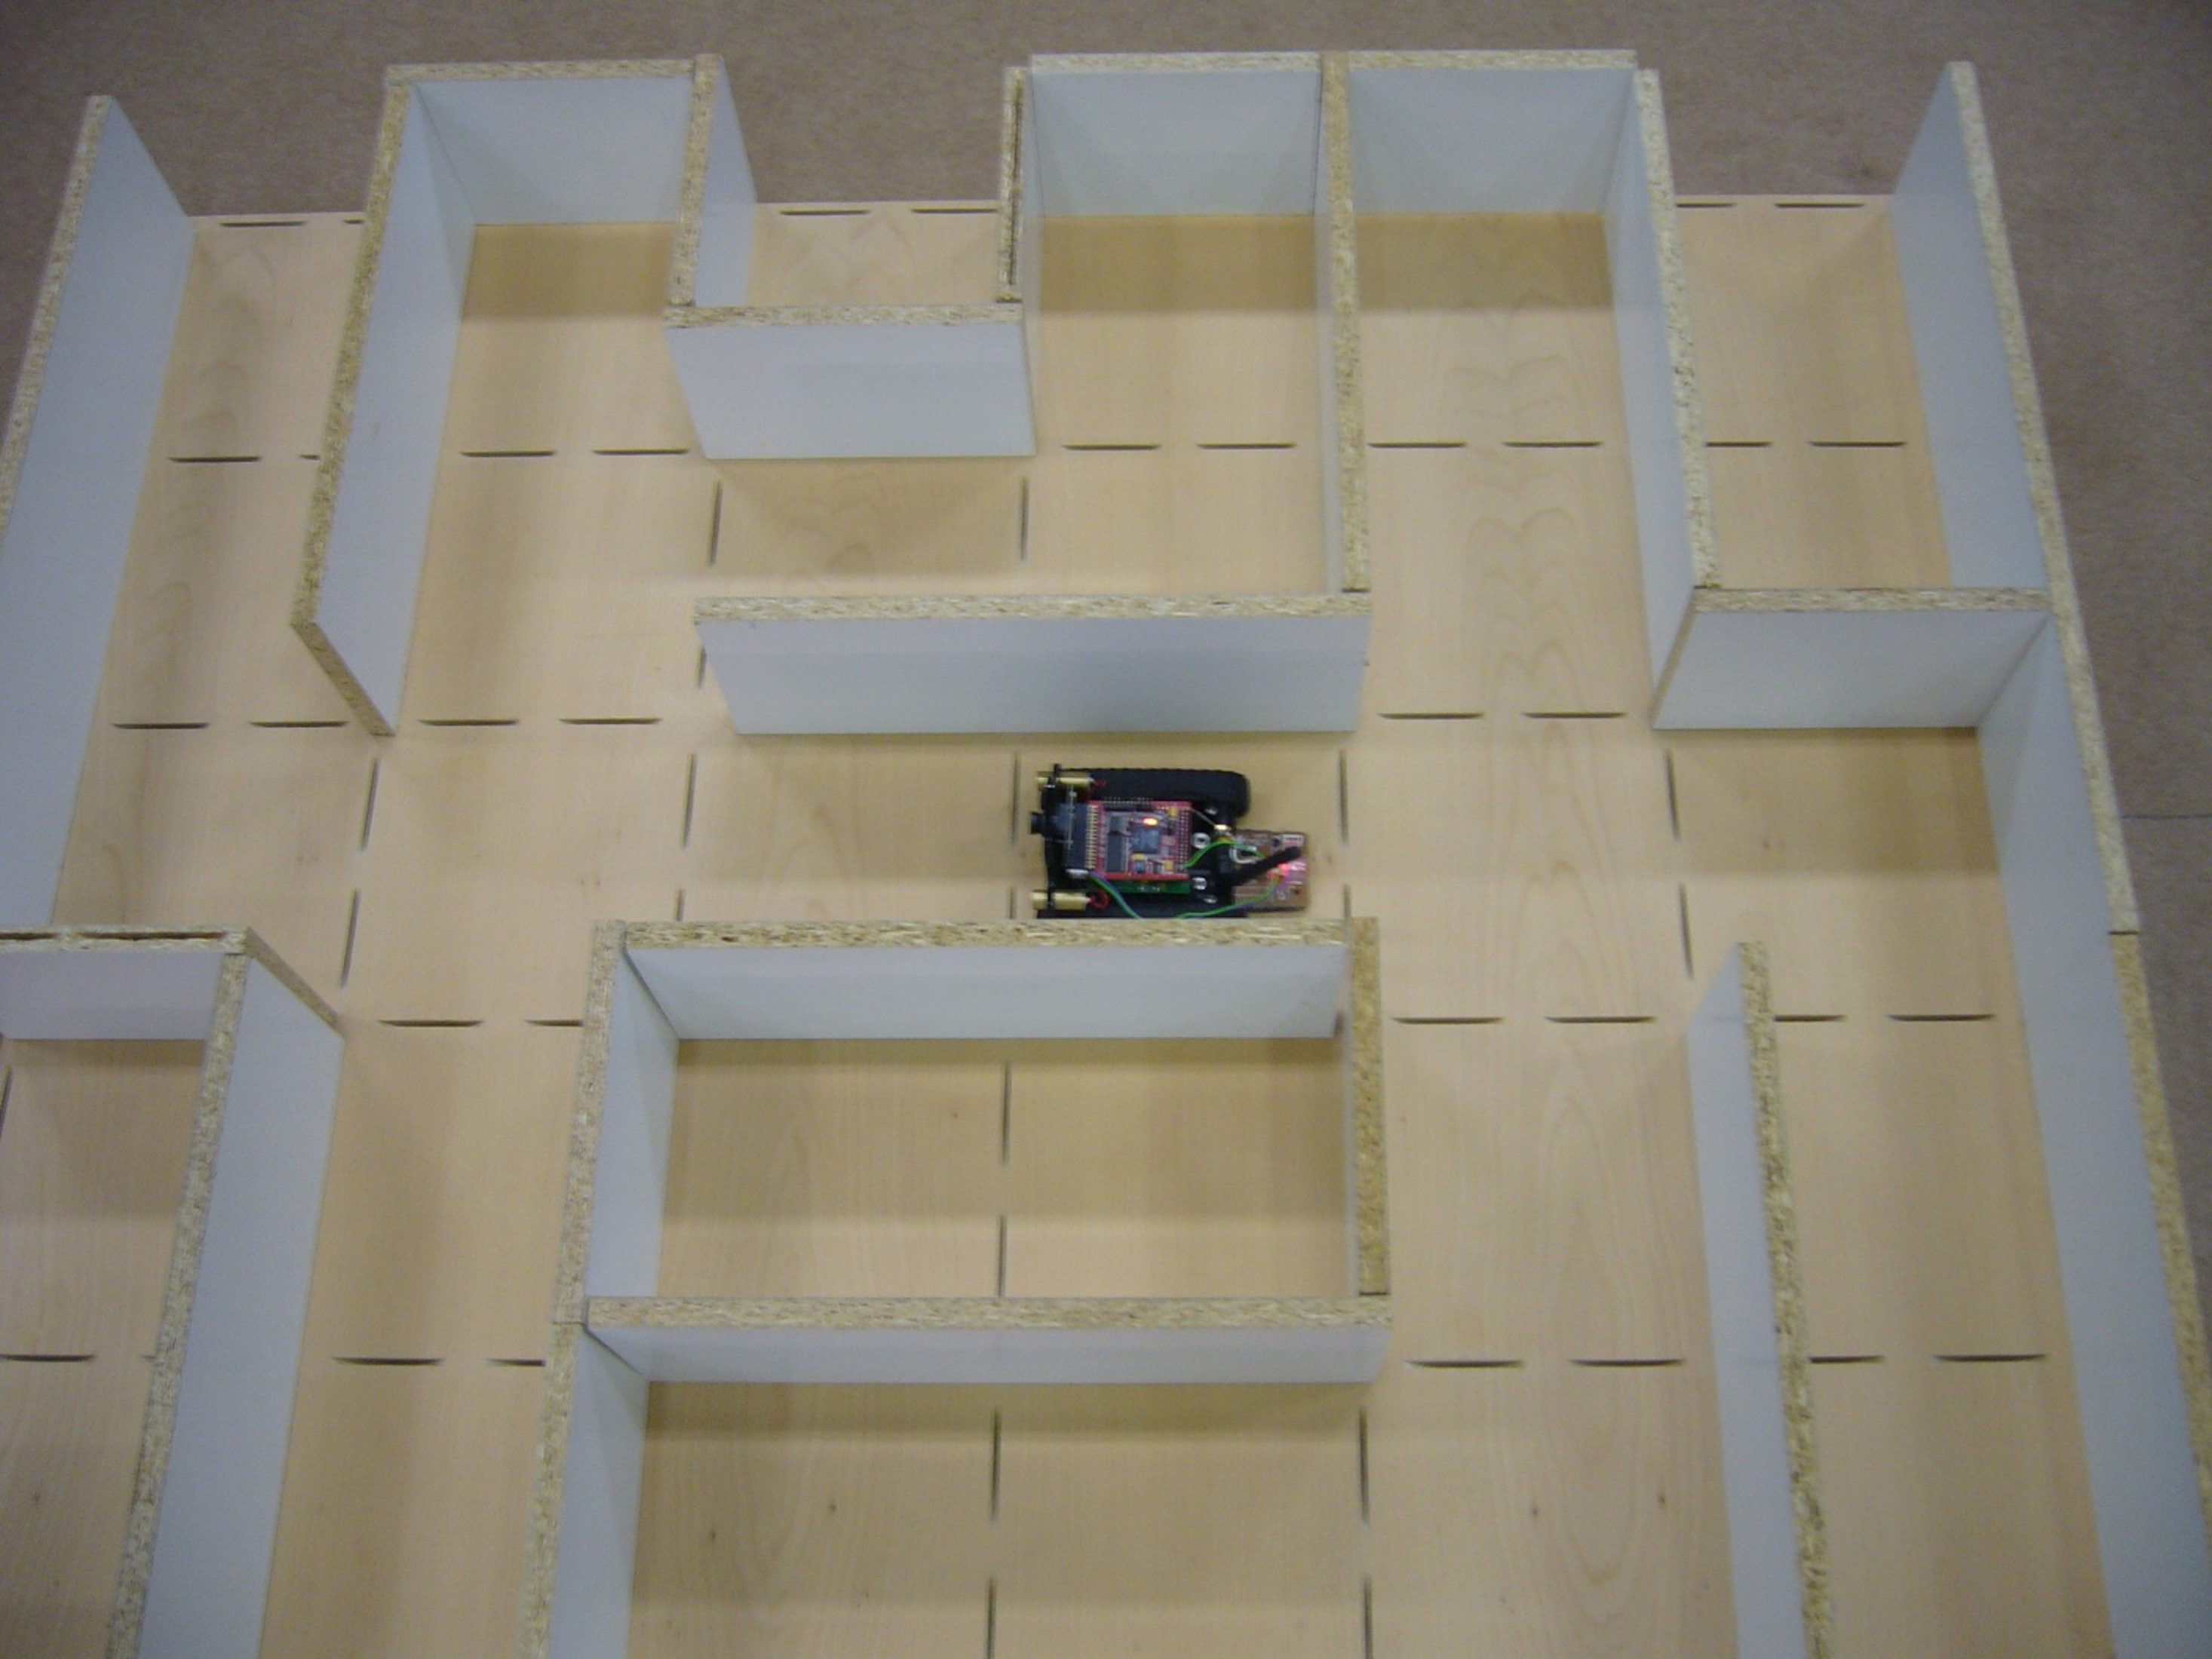
\includegraphics[width=0.45\columnwidth]{diagrams/maze.pdf}
	}
\caption{(a), (b): Different types of grid maps. (c), (d):
Some common application areas.}
 \end{figure}
